\section{Countable Sets}\label{S:infinitesets}
%\markboth{Chapter~\ref{C:topicsinsets}. Topics in Set Theory}{\ref{S:infinitesets}. Countable 
%Sets}
\setcounter{previewactivity}{0}
%
\begin{previewactivity}[\textbf{Introduction to Infinite Sets}]\label{PA:introtoinfinite} \hfill \\
In Section~\ref{S:finitesets}, we defined a \textbf{finite set}
\index{finite set}%
 to be the empty set or a set $A$ such that $A \approx \mathbb{N}_k$ for some natural number $k$.    We also defined an 
\textbf{infinite set} 
\index{infinite set}%
to be a set that is not finite, but the question now is, ``How do we know if a set is infinite?''  
One way to determine if a set is an infinite set is to use 
Corollary~\ref{C:propersubsets}, which states that a finite set is not equivalent to any of its subsets.  We can write this as a conditional statement as follows:

\begin{list}{}
\item If $A$ is a finite set, then $A$ is not equivalent to any of its proper subsets.
\end{list}
\noindent
or more formally as
\begin{list}{}
\item For each set $A$, if $A$ is a finite set, then for each proper subset $B$ of $A$, $A \not\approx B$.
\end{list}

\begin{enumerate}
\item Write the contrapositive of the preceding conditional statement.  Then explain how this statement can be used to determine if a set is infinite.

\item Let $D^+$ be the set of all odd natural numbers.  In \typeu Activity~\ref*{PA:equivalentsets} from Section~\ref{S:finitesets}, we proved that $\mathbb{N} \approx D^+$. 
\label{PA:introtoinfinite2}%

\begin{enumerate}
\item Use this to explain carefully why $\mathbb{N}$ is an infinite set.

\item Is $D^+$ a finite set or an infinite set?  Explain carefully  how you know.
\end{enumerate}

\item Let $b$ be a positive real number.  Let $( 0, 1 )$ and 
$( 0, b )$ be the open intervals from 0 to 1 and 0 to $b$, respectively.  In 
Part~(\ref{A:equivsets4}) of Progress Check~\ref{prog:equivsets} 
(on page~\pageref{prog:equivsets}), 
%Beginning Activity~\ref{PA:equivalentsets} from Section~\ref{S:finitesets}, 
we proved that 
$( 0, 1 ) \approx ( 0, b )$. 
\label{PA:introtoinfinite3}%

\begin{enumerate}
\item Use a value for $b$ where $0 < b < 1$ to explain why $( 0, 1 )$ is an infinite set.

\item Use a value for $b$ where $b > 1$ to explain why $( 0, b )$ is an infinite set.
\end{enumerate}

\end{enumerate}
\end{previewactivity}
%\hbreak

\endinput




\begin{previewactivity}[\textbf{A Function from $\boldsymbol{\N}$ to $\boldsymbol{\Z}$}]\label{PA:functionNtoZ} \hfill \\
In this activity, we will define and explore a function $f:\mathbb{N} \to \mathbb{Z}$.  We will start by defining $f ( n )$ for the first few natural numbers $n$.

\begin{center}
\begin{tabular}[h]{l p{2cm} l}
$f ( 1 ) = 0$  &  &  \\
$f ( 2 ) = 1$  &  &  $f ( 3 ) = -1$ \\
$f ( 4 ) = 2$  &  &  $f ( 5 ) = -2$ \\
$f ( 6 ) = 3$  &  &  $f ( 7 ) = -3$\\
\end{tabular}
\end{center}
Notice that if we list the outputs of $f$ in the order 
$f ( 1 ), f ( 2 ), f ( 3 ), \ldots$,  we create the following list of integers:
$0, 1, -1, 2, -2, 3, -3, \ldots$.  We can also illustrate the outputs of this function with the following diagram:
\begin{figure}[h]
$$
\BeginTable
\BeginFormat
| c | c | c | c | c | c | c | c | c | c | c |
\EndFormat
" 1 " 2 " 3 " 4 " 5 " 6 " 7 " 8 " 9 " 10 " $\cdots$ " \\
" $\downarrow$ " $\downarrow$ " $\downarrow$ " $\downarrow$ " $\downarrow$ " $\downarrow$ " $\downarrow$ " $\downarrow$ " $\downarrow$ " $\downarrow$ " $\cdots$ "\\
" 0 " 1 " $-1$ " 2 " $-2$ " 3 " $-3$ " 4 " $-4$ " 5 "  $\cdots$ " \\
\EndTable
$$
\caption{A Function from $\N$ to $\Z$} \label{fig:functionNtoZ}
\end{figure}


\begin{enumerate}
\item If the pattern suggested by the function values we have defined continues, what are 
$f ( 11 )$ and $f ( 12 )$?  What is $f ( n )$ for $n$ from 13 to 16? 
\label{PA:functionNtoZ1}%

\item If the pattern of outputs continues, does the function $f$ appear to be an injection?  Does $f$ appear to be a surjection?  (Formal proofs are not required.)
\end{enumerate}

We will now attempt to determine a formula for $f ( n )$, where $n \in \mathbb{N}$.  We will actually determine two formulas:  one for when $n$ is even and one for when $n$ is odd.

\begin{enumerate} \setcounter{enumi}{2}
\item Look at the pattern of the values of $f ( n )$ when $n$ is even.  What appears to be a formula for $f ( n )$ when $n$ is even? 
\label{PA:functionNtoZ3}%

\item Look at the pattern of the values of $f ( n )$ when $n$ is odd.  What appears to be a formula for $f ( n )$ when $n$ is odd? 
\label{PA:functionNtoZ4}%

\item Use the work in Part~(\ref{PA:functionNtoZ3}) and Part~(\ref{PA:functionNtoZ4}) to complete the following:  Define $f\x \mathbb{N} \to \mathbb{Z}$, where
\[
f ( n ) = \left\{ \begin{gathered}
  ?? \text{  if  }n \text{ is even} \hfill \\
\\
  ?? \text{  if  }n \text{ is odd}. \hfill \\ 
\end{gathered}  \right.
\]
\label{PA:functionNtoZ5}%

\item Use the formula in Part~(\ref{PA:functionNtoZ5}) to
\begin{enumerate}
\item Calculate $f ( 1 )$ through $f ( 10 )$.  Are these results consistent with the pattern exhibited at the start of this activity?

\item Calculate $f ( 1000 )$ and $f ( 1001 )$.

\item Determine the value of $n$ so that $f ( n ) = 1000$.
\end{enumerate}
\end{enumerate} 
\end{previewactivity}
\hbreak

\endinput

%
In this section, we will describe several infinite sets and define the cardinal number for so-called countable sets.  Most of our examples will be subsets of some of our standard number systems such as $\mathbb{N}$, $\mathbb{Z}$, and $\mathbb{Q}$.  

%We will see that there are infinite sets that may appear to be different in size, and that there exist infinite sets that are not equivalent.

\subsection*{Infinite Sets}
In \typeu Activity~\ref*{PA:introtoinfinite}, we saw how to use Corollary~\ref{C:propersubsets} to prove that a set is infinite.  This corollary implies that if $A$ is a finite set, then $A$ is not equivalent to any of its proper subsets.  By writing the contrapositive of this conditional statement, we can restate Corollary~\ref{C:propersubsets} in the following form:

\vskip9pt
\noindent
\textbf{Corollary~\ref{C:propersubsets}}.
\emph{If a set $A$ is equivalent to one of its proper subsets, then $A$ is infinite.}

%\begin{theorem} \label{T:infinitesets}
%The set $A$ is an infinite set if and only if $A$ is equivalent to one of its proper subsets.
%\end{theorem}

%\begin{example} 
\newpar
In \typeu Activity~\ref*{PA:introtoinfinite}, we used Corollary~\ref{C:propersubsets} to prove that
\begin{itemize}
\item The set of natural numbers, $\mathbb{N}$, is an infinite set.

\item The open interval $( 0, 1 )$ is an infinite set.
\end{itemize}
%\end{example}
Although Corollary~\ref{C:propersubsets} provides one way to prove that a set is infinite, it is sometimes more convenient to use a proof by contradiction to prove that a set is infinite.  The idea is to use results from Section~\ref{S:finitesets} about finite sets to help obtain a contradiction.  This is illustrated in the next theorem.
\begin{theorem}\label{T:subsetisinfinite}
Let $A$ and $B$ be sets.
\begin{enumerate}
\item If $A$ is infinite and $A \approx B$, then $B$ is infinite.  \label{T:subsetisinfinite1}
\item If $A$ is infinite and $A \subseteq B$, then $B$ is infinite.  \label{T:subsetisinfinite2}
\end{enumerate}
\end{theorem}
%
\begin{myproof}
We will prove part~(\ref{T:subsetisinfinite1}).  The proof of part~(\ref{T:subsetisinfinite2}) is exercise~(\ref{exer:subsetisinfinite}) on page~\pageref{exer:subsetisinfinite}.

To prove part~(\ref{T:subsetisinfinite1}), we use a proof by contradiction and assume that $A$ is an infinite set, $A \approx B$, and $B$ is not infinite.  That is, $B$ is a finite set.  Since $A \approx B$ and $B$ is finite, Theorem~\ref{T:equivfinitesets} on page~\pageref{T:equivfinitesets} implies that $A$ is a finite set.  This is a contradiction to the assumption that $A$ is infinite.  We have therefore proved that if $A$ is infinite and $A \approx B$, then $B$ is infinite.
\end{myproof}

%\begin{activity}[Proof of Theorem~\ref{T:subsetisinfinite}] \label{A:subsetisfinite}
%Write a proof for both parts of Theorem~\ref{T:subsetisinfinite}.  For both parts, use a proof by contradiction.  For each proof, a theorem in Section~\ref{S:finitesets} will provide a contradiction.
%\end{activity}
\hbreak
%
%\begin{example}[Examples of Infinite Sets] \label{E:infinitesets} \hfill
%\begin{itemize}
%\item Theorem~\ref{T:subsetisinfinite} allows us to conclude that our standard number systems are infinite sets since they all have $\mathbb{N}$ as a subset.  So $\mathbb{Z}$, $\mathbb{Q}$, and $\mathbb{R}$ are all infinite sets.  In addition, the set of all positive rational numbers, 
%$\mathbb{Q}^+$, and the set of all positive real numbers, $\mathbb{R}^+$, are infinite sets.
%
%\item Let $D^+$ be the set of all odd natural numbers.  In Part~(\ref{PA:introtoinfinite2}) of Beginning Activity~\ref{PA:introtoinfinite}, we proved that $D^+ \approx \mathbb{N}$.  Therefore, by Theorem~\ref{T:subsetisinfinite}, $D^+$ is an infinite set.  In a similar manner, the set $E^+$ of all even natural numbers is an infinite set.  To do this, we can use the function $g\x \mathbb{N} \to E^+$ defined by $g ( x ) = 2x$ for all $x \in \mathbb{N}$.
%\end{itemize}
%\end{example}
\begin{prog}[\textbf{Examples of Infinite Sets}] \label{E:infinitesets} \hfill
\begin{enumerate}
\item In \typeu Activity~\ref*{PA:introtoinfinite}, we used Corollary~\ref{C:propersubsets} to prove that $\N$ is an infinite set.  Now use this and Theorem~\ref{T:subsetisinfinite} to explain why our standard number systems $( \Z, \Q, \text{ and } \R )$ are infinite sets.  Also, explain why the set of all positive rational numbers, 
$\Q^+$, and the set of all positive real numbers, $\R^+$, are infinite sets.

\item Let $D^+$ be the set of all odd natural numbers.  In Part~(\ref{PA:introtoinfinite2}) of \typeu Activity~\ref*{PA:introtoinfinite}, we proved that $D^+ \approx \mathbb{N}$.  Use 
Theorem~\ref{T:subsetisinfinite} to explain why $D^+$ is an infinite set.  

\item Prove that the set $E^+$ of all even natural numbers is an infinite set.
\end{enumerate}
\end{prog}
\hbreak

\endinput


\subsection*{Countably Infinite Sets}
In Section~\ref{S:finitesets}, we used the set $\mathbb{N}_k$ as the standard set with cardinality $k$ in the sense that a set is finite if and only if it is equivalent to 
$\mathbb{N}_k$.  In a similar manner, we will use some infinite sets as standard sets for certain infinite cardinal numbers.  The first set we will use is $\mathbb{N}$.  

We will formally define what it means to say the elements of a set can be ``counted'' using the natural numbers.  The elements of a finite set can be ``counted'' by defining a bijection (one-to-one correspondence) between the set and $\mathbb{N}_k$ for some natural number $k$.  We will be able to ``count'' the elements of an infinite set if we can define a one-to-one correspondence between the set and $\mathbb{N}$.

\begin{defbox}{aleph0}{The \textbf{cardinality of} $\boldsymbol{\mathbb{N}}$
\index{cardinality}%
\index{cardinality!natural numbers}%
\index{cardinality!$\aleph_0$}%
%\index{$\aleph_0$}%
 is denoted by $\aleph_0$.  
\label{sym:aleph0}%
 The symbol $\aleph$ is the first letter of the Hebrew alphabet, \textbf{aleph}.
\index{aleph}%
  The subscript 0 is often read as ``naught'' (or sometimes as ``zero'' or ``null'').  So we write
\[
\text{card}( \N ) = \aleph_0
\]
and say that the cardinality of $\mathbb{N}$ is ``aleph naught.''}
\end{defbox}
%
\begin{defbox}{countinfinite}{A set $A$ is \textbf{countably infinite}
\index{countably infinite set}%
 provided that 
$A \approx \mathbb{N}$.  In this case, we write
\[
\text{card}( A ) = \aleph_0.
\]
A set that is countably infinite is sometimes called a \textbf{denumerable}
\index{denumerable set}%
 set.  A set is 
\textbf{countable}
\index{countable set}%
 provided that it is finite or countably infinite.  An infinite set that is not countably infinite is called an \textbf{uncountable set}.
\index{uncountable set}%
}
\end{defbox}
%
\begin{prog}[\textbf{Examples of Countably Infinite Sets}]\label{prog:countablyinfinitesets} \hfill
\begin{enumerate}
\item In \typeu Activity~\ref*{PA:equivalentsets} from Section~\ref{S:finitesets}, we proved that 
$\mathbb{N} \approx D^+$, where $D^+$ is the set of all odd natural numbers.  Explain why 
$\text{card}( D^+ ) = \aleph_0$.

\item Use a result from Progress Check~\ref{E:infinitesets} to explain why 
$\text{card}( E^+ ) = \aleph_0$.

\item At this point, if we wish to prove a set $S$ is countably infinite, we must find a bijection between the set $S$ and some set that is known to be countably infinite.

Let $S$ be the set of all natural numbers that are perfect squares.  Define a function 
\[
f\x S \to \mathbb{\N}
\]
that can be used to prove that $S \approx \mathbb{N}$ and, hence, that 
$\text{card}( S ) = \aleph_0$.
\end{enumerate}
\end{prog}\hbreak
%
The fact that the set of integers is a countably infinite set is important enough to be called a theorem.  The function we will use to establish that $\N \approx \Z$ was explored in \typeu Activity~\ref*{PA:functionNtoZ}.

\begin{theorem}\label{T:ZequivtoN}
The set $\Z$ of integers is countably infinite, and so 
$\text{card}( \Z ) = \aleph_0$.
\end{theorem}
%
\begin{myproof}
To prove that $\N \approx \Z$, we will use the following function:
$f\x \N \to \Z$, where
%
\begin{equation} \notag
f ( n ) = 
\begin{cases}
\dfrac{n}{2}         &\text{if $n$ is even} \\
                      &                      \\
\dfrac{1-n}{2}       &\text{if $n$ is odd}.
\end{cases}
\end{equation}
%
From our work in \typeu Activity~\ref*{PA:functionNtoZ}, it appears that if $n$ is an even natural number, then $f ( n ) > 0$, and if $n$ is an odd natural number, then 
$f ( n ) \leq 0$.  So it seems reasonable to use cases to prove that $f$ is a surjection and that $f$ is an injection.
To prove that $f$ is a surjection, we let $y \in \mathbb{Z}$.
\begin{itemize}
\item If $y > 0$, then $2y \in \mathbb{N}$, and
\[
f ( 2y ) = \frac{2y}{2} = y.
\]
\item If $y \leq 0$, then $-2y \geq 0$ and $1 - 2y$ is an odd natural number.  Hence,
\[
f ( 1 - 2y ) = \frac{1 - (1 - 2y )}{2} = \frac{2y}{2}=y.
\]
\end{itemize}
These two cases prove that if $y \in \mathbb{Z}$, then there exists an $n \in \mathbb{N}$ such that \linebreak
$f ( n ) = y$.  Hence, $f$ is a surjection.

\vskip6pt
To prove that $f$ is an injection, we let $m, n \in \mathbb{N}$ and assume that  
$f ( m ) = f ( n )$.  First note that if one of $m$ and $n$ is odd and the other is even, then one of $f ( m )$ and $f ( n )$ is positive and the other is less than or equal to 0.  So if $f ( m ) = f ( n )$, then both $m$ and $n$ must be even or both $m$ and $n$ must be odd.
\begin{itemize}
\item If both $m$ and $n$ are even, then
\begin{center}
$f ( m ) = f ( n )$ implies that $\dfrac{m}{2} = \dfrac{n}{2}$
\end{center}
and hence that $m = n$.

\item If both $m$ and $n$ are odd, then
\begin{center}
$f ( m ) = f ( n )$ implies that $\dfrac{1-m}{2} = \dfrac{1-n}{2}$.
\end{center}
From this, we conclude that $1 - m$ = $1 - n$ and hence that $m = n$.  This proves that if 
$f ( m ) = f ( n )$, then $m = n$ and hence that $f$ is an injection.
\end{itemize}

Since $f$ is both a surjection and an injection, we see that $f$ is a bijection and, therefore, 
$\mathbb{N} \approx \mathbb{Z}$.  Hence, $\mathbb{Z}$ is countably infinite and
$\text{card} ( \Z ) = \aleph_0$.
\end{myproof}

The result in Theorem~\ref{T:ZequivtoN} can seem a bit surprising.  It exhibits one of the distinctions between finite and infinite sets.  If we add elements to a finite set, we will increase its size in the sense that the new set will have a greater cardinality than the old set.  However, with infinite sets, we can add elements and the new set may still have the same cardinality as the original set.  For example, there is a one-to-one correspondence between the elements of the sets $\N$ and $\Z$.  We say that these sets have the same cardinality.

Following is a summary of some of the main examples dealing with the cardinality of sets that we have explored.

\begin{itemize}
\item The sets $\mathbb{N}_k$, where $k \in \mathbb{N}$, are examples of sets that are countable and finite.
\item The sets $\mathbb{N}$, $\mathbb{Z}$, the set of all odd natural numbers, and the set of all even natural numbers are examples of sets that are countable and countably infinite.
\item We have not yet proved that any set is uncountable.
\end{itemize}

%

\endinput

\subsection*{The Set of Positive Rational Numbers}
If we expect to find an uncountable set in our usual number systems, the rational numbers might be the place to start looking.  One of the main differences between the set of rational numbers and the integers is that given any integer $m$, there is a next integer, namely $m + 1$.  This is not true for the set of rational numbers.  We know that $\Q$ is closed under division (by nonzero rational numbers) and we will see that this property implies that given any two rational numbers, we can also find a rational number between them.  In fact, between any two rational numbers, we can find infinitely many rational numbers.  It is this property that may lead us to believe that there are ``more'' rational numbers than there are integers.

The basic idea will be to ``go half way'' between two rational numbers.  For example, if we use $a = \dfrac{1}{3}$ and $b = \dfrac{1}{2}$, we can use
\[
\frac{a+b}{2} = \frac{1}{2} \left( \frac{1}{3} + \frac{1}{2} \right) = \frac{5}{12}
\]
as a rational number between $a$ and $b$.  We can then repeat this process to find a rational number between 
$\dfrac{5}{12}$ and $\dfrac{1}{2}$.

So we will now let $a$ and $b$ be any two rational numbers with $a < b$ and let $c_1 = \dfrac{a+b}{2}$.  We then see that%
\label{tworationals}%
\begin{align*}
c_1 - a &= \frac{a+b}{2} - a &  b- c_1 &= b - \frac{a+b}{2} \\
        &= \frac{a+b}{2} - \frac{2a}{2} &  &= \frac{2b}{2} - \frac{a+b}{2} \\
        &= \frac{b-a}{2}                &  &= \frac{b-a}{2}
\end{align*}
Since $b > a$, we see that $b - a > 0$ and so the previous equations show that $c_1 - a > 0$ and $b - c_1 > 0$.  We can then conclude that $a < c_1 < b$.

We can now repeat this process by using $c_2 = \dfrac{c_1 + b}{2}$ and proving that $c_1 < c_2 < b$.  In fact, for each natural number, we can define
\[
c_{k + 1} = \frac{c_k + b}{2}
\]
and obtain the result that $a < c_1 < c_2 < \cdots < c_n < \cdots < b$ and this proves that the set 
$\left\{ c_k \mid k \in \mathbb{N} \right\}$ is a countably infinite set where each element is a rational number between $a$ and $b$.  (A formal proof can be completed using mathematical induction.)  See Exercise~(\ref{exer:tworationals}).

This result is true no matter how close together $a$ and $b$ are.  For example, we can now conclude that there are infinitely many rational numbers between 0 and $\dfrac{1}{10000}$.  This might suggest that the set $\mathbb{Q}$ of rational numbers is uncountable.  Surprisingly, this is not the case.  We start with a proof that the set of positive rational numbers is countable.

\begin{theorem}\label{T:positiverationals}
The set of positive rational numbers is countably infinite.
\end{theorem}
%
\begin{myproof}
We can write all the positive rational numbers in a two-dimensional array as shown in 
Figure~\ref{fig:positiverationals}.
%
\begin{figure}[h]
\begin{center}
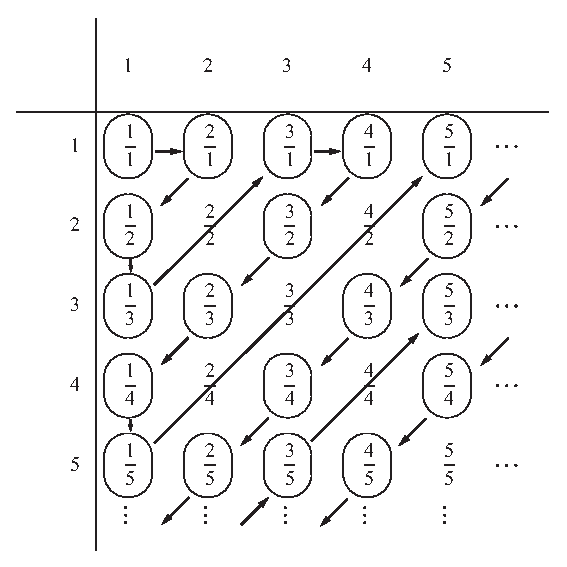
\includegraphics{figps-rationals.eps}
\caption{Counting the Positive Rational Numbers}\label{fig:positiverationals}
\end{center}
\end{figure}
The top row in Figure~\ref{fig:positiverationals} represents the numerator of the rational number, and the left column represents the denominator.  We follow the arrows in 
Figure~\ref{fig:positiverationals} to define $f\x \mathbb{N} \to \mathbb{Q}^+$.  The idea is to start in the upper left corner of the table and move to successive diagonals  as follows:
\begin{itemize}
\item We start with all fractions in which the sum of the numerator and denominator is 2 
$\left( \text{only } \dfrac{1}{1} \right)$.  So $f ( 1 ) = \dfrac{1}{1}$.

\item We next use those fractions in which the sum of the numerator and denominator is 3.  So 
$f ( 2 ) = \dfrac{2}{1}$ and $f ( 3 ) = \dfrac{1}{2}$.

\item We next use those fractions in which the sum of the numerator and denominator is 4.  So 
$f ( 4 ) = \dfrac{1}{3}$, $f ( 5 ) = \dfrac{3}{1}$.  We skipped 
$\dfrac{2}{2}$ since $\dfrac{2}{2} = \dfrac{1}{1}$.  In this way, we will ensure that the function $f$ is a one-to-one function.
\end{itemize}
We now continue with successive diagonals omitting fractions that are not in lowest terms.  This process guarantees that the function $f$ will be an injection and a surjection.  Therefore, 
$\mathbb{N} \approx \mathbb{Q}^+$ and $\text{card} ( \mathbb{Q}^+ ) = \aleph_0$.
\end{myproof}

\newpar
\note For another proof of Theorem~\ref{T:positiverationals}, see exercise~(\ref{A:Qcountable}) on page~\pageref{A:Qcountable}.

\newpar
Since $\mathbb{Q}^+$ is countable, it seems reasonable to expect that $Q$ is countable.  We will explore this soon.  On the other hand, at this point, it may also seem reasonable to ask, 
\begin{center}
``Are there any uncountable sets?''
\end{center}
The answer to this question is yes, but we will wait until the next section to prove that certain sets are uncountable.  We still have a few more issues to deal with concerning countable sets.
\endinput

\subsection*{Countably Infinite Sets}

\begin{theorem}\label{T:addonetocountable}
If $A$ is a countably infinite set, then $A \cup \left\{ x \right\}$ is a countably infinite set.
\end{theorem}
%
\begin{myproof}
Let $A$ be a  countably infinite set.  Then there exists a bijection $f\x \mathbb{N} \to A$.  Since $x$ is either in $A$ or not in $A$, we can consider two cases.

\newpar
If $x \in A$, then $A \cup \left\{ x \right\} = A$ and $A \cup \left\{ x \right\}$ is countably infinite.

\newpar
If $x \notin A$, define $g\x \mathbb{N} \to A \cup \left\{ x \right\}$ by
\begin{equation} \notag
g( n ) = 
\begin{cases}
x                        &\text{if $n = 1$} \\
f ( n - 1 )   &\text{if $n > 1$.}
\end{cases}
\end{equation}
The proof that the function $g$ is a bijection is Exercise~(\ref{exer:addonetocountable}).  Since $g$ is a bijection, we have proved that $A \cup \left\{ x \right\} \approx \N$ and hence, $A \cup \left\{ x \right\}$ is countably infinite.
\end{myproof}
%
\begin{theorem}\label{T:addfinitetocountable}
If $A$ is a countably infinite set and $B$ is a finite set, then $A \cup B$ is a countably infinite set.
\end{theorem}
%
\begin{myproof}
Exercise~(\ref{exer:addfinitetocountable}) on page~\pageref{exer:addfinitetocountable}.
\end{myproof}
%

Theorem~\ref{T:addfinitetocountable} says that if we add a finite number of elements to a countably infinite set, the resulting set is still countably infinite.  In other words, the cardinality of the new set is the same as the cardinality of the original set.  Finite sets behave very differently in the sense that if we add elements to a finite set, we will change the cardinality.  What may even be more surprising  is the result in Theorem~\ref{T:unionofcountable} that states that the union of two countably infinite (disjoint) sets is countably infinite.  The proof of this result is similar to the proof that the integers are countably infinite  (Theorem~\ref{T:ZequivtoN}).  In fact, if $A = \{a_1, a_2, a_3, \ldots \}$ and $B = \{b_1, b_2, b_3, \ldots \}$, then we can use the following diagram to help define a bijection from $\N$ to $A \cup B$.


\begin{figure}[h]
$$
\BeginTable
\BeginFormat
| c | c | c | c | c | c | c | c | c | c | c |
\EndFormat
" 1 " 2 " 3 " 4 " 5 " 6 " 7 " 8 " 9 " 10 " $\cdots$ " \\
" $\downarrow$ " $\downarrow$ " $\downarrow$ " $\downarrow$ " $\downarrow$ " $\downarrow$ " $\downarrow$ " $\downarrow$ " $\downarrow$ " $\downarrow$ " $\cdots$ "\\
" $a_1$ " $b_1$ " $a_2$ " $b_2$ " $a_3$ " $b_3$ " $a_4$ " $b_4$ " $a_5$ " $b_5$ "  $\cdots$ " \\
\EndTable
$$
\caption{A Function from $\N$ to $A \cup B$} \label{fig:functionNtoUnion}
\end{figure}


\begin{theorem}\label{T:unionofcountable}
If $A$ and $B$ are disjoint countably infinite sets,
\index{countably infinite sets!union of}%
 then $A \cup B$ is a countably infinite set.
\end{theorem}
%
\begin{myproof}
Let $A$ and $B$ be countably infinite sets and let $f\x \mathbb{N} \to A$ and 
$g\x \mathbb{N} \to B$ be bijections.  Define $h\x \mathbb{N} \to A \cup B$ by
\begin{equation} \notag
h( n ) = 
\begin{cases}
f \!\left( \dfrac{n+1}{2} \right)                        &\text{if $n$ is odd} \\
                                                       & \\
g \!\left( \dfrac{n}{2} \right)                          &\text{if $n$ is even}.
\end{cases}
\end{equation}
It is left as Exercise~(\ref{exer:unionofcountable}) on 
page~\pageref{exer:unionofcountable} to prove that the function $h$ is a bijection.
\end{myproof}

Since we can write the set of rational numbers $\Q$ as the union of the set of nonnegative rational numbers and the set of negative rational numbers, we can use the results in Theorem~\ref{T:positiverationals}, Theorem~\ref{T:addonetocountable}, and Theorem~\ref{T:unionofcountable} to prove the following theorem.

\begin{theorem}\label{T:Qiscountable}
The set $\mathbb{Q}$ of all rational numbers is countably infinite.
\end{theorem}
%
\begin{myproof}
Exercise~(\ref{exer:Qiscountable}) on page~\pageref{exer:Qiscountable}.
\end{myproof}
%\hbreak
%
\index{countably infinite sets!subsets of|(}%
In Section~\ref{S:finitesets}, we proved that any subset of a finite set is finite 
(Theorem~\ref{T:finitesubsets}).  A similar result should be expected for countable sets. We first prove that every subset of $\mathbb{N}$ is countable.  For an infinite subset $B$ of 
$\mathbb{N}$, the idea of the proof is to define a function $g\x  \mathbb{N} \to B$ by removing the elements from $B$ from smallest to the next smallest to the next smallest, and so on.  
We do this by defining the function $g$ recursively as follows:
\begin{itemize}
\item Let $g ( 1 )$ be the smallest natural number in $B$.
\item Remove $g ( 1 )$ from $B$ and let $g ( 2 )$ be the smallest natural number in \linebreak
$B - \left\{ g ( 1 ) \right\}$.
\item Remove $g ( 2 )$ and let $g ( 3 )$ be the smallest natural number in 
\linebreak
$B - \left\{ g ( 1 ), g ( 2 ) \right\}$.
\item We continue this process.  The formal recursive definition of $g\x  \mathbb{N} \to B$ is included in the proof of Theorem~\ref{T:subsetsofN}.
\end{itemize}
%
\begin{theorem}\label{T:subsetsofN}
Every subset of the natural numbers is countable.
\end{theorem}
%
\begin{myproof}
Let $B$ be a subset of $\mathbb{N}$.  If $B$ is finite, then $B$ is countable.  So we next assume that $B$ is infinite.  We will next give a recursive definition of a function 
$g\x  \mathbb{N} \to B$ and then prove that $g$ is a bijection.
\begin{itemize}
\item Let $g ( 1 )$ be the smallest natural number in $B$.
\item For each $n \in \mathbb{N}$, the set 
$B - \left\{ g ( 1 ), g ( 2 ), \ldots, g ( n ) \right\}$ is not empty since $B$ is infinite.  Define $g ( n + 1 )$ to be the smallest natural number in 
\linebreak
$B - \left\{ g ( 1 ), g ( 2 ), \ldots, g ( n ) \right\}$.
\end{itemize}
The proof that the function $g$ is a bijection is Exercise~(\ref{exer:subsetofN}) on page~\pageref{exer:subsetofN}.  
\end{myproof}
%
\begin{corollary}\label{C:subsetofcountable}
Every subset of a countable set is countable.
\end{corollary}
%
\begin{myproof}
Exercise~(\ref{exer:subsetofcountable}) on page~\pageref{exer:subsetofcountable}.
\end{myproof}
\index{countably infinite sets!subsets of|)}%

\hbreak

\endinput


\endinput



%\hrule
%

Since $\mathbb{Q}^+$ is countable, it seems reasonable to expect that $Q$ is countable.  We will explore this soon.  On the other hand, at this point, it may also seem reasonable to ask, 
\begin{center}
``Are there any uncountable sets?''
\end{center}

\begin{figure}[h]
\begin{center}
\setlength{\unitlength}{0.5cm}
\begin{picture}(20,20)
\put(4,18){1}
\put(7,18){2}
\put(10,18){3}
\put(13,18){4}
\put(16,18){5}

\put(2,15){1}
\put(2,12){2}
\put(2,9){3}
\put(2,6){4}
\put(2,3){5}

\put(0,16.5){\line(1,0){20}}
\put(3,0){\line(0,1){20}}

\put(4,15){$\dfrac{1}{1}$}
\put(7,15){$\dfrac{2}{1}$}
\put(10,15){$\dfrac{3}{1}$}
\put(13,15){$\dfrac{4}{1}$}
\put(16,15){$\dfrac{5}{1}$}
\put(18,15){$\cdots$}

\put(4.2,15.2){\oval(1.8,2.4)}
\put(7.2,15.2){\oval(1.8,2.4)}
\put(10.2,15.2){\oval(1.8,2.4)}
\put(13.2,15.2){\oval(1.8,2.4)}
\put(16.2,15.2){\oval(1.8,2.4)}

\put(4,12){$\dfrac{1}{2}$}
\put(7,12){$\dfrac{2}{2}$}
\put(10,12){$\dfrac{3}{2}$}
\put(13,12){$\dfrac{4}{2}$}
\put(16,12){$\dfrac{5}{2}$}
\put(18,12){$\cdots$}

\put(4.2,12.2){\oval(1.8,2.4)}
\put(10.2,12.2){\oval(1.8,2.4)}
\put(16.2,12.2){\oval(1.8,2.4)}

\put(4,9){$\dfrac{1}{3}$}
\put(7,9){$\dfrac{2}{3}$}
\put(10,9){$\dfrac{3}{3}$}
\put(13,9){$\dfrac{4}{3}$}
\put(16,9){$\dfrac{5}{3}$}
\put(18,9){$\cdots$}

\put(4.2,9.2){\oval(1.8,2.4)}
\put(7.2,9.2){\oval(1.8,2.4)}
\put(13.2,9.2){\oval(1.8,2.4)}
\put(16.2,9.2){\oval(1.8,2.4)}

\put(4,6){$\dfrac{1}{4}$}
\put(7,6){$\dfrac{2}{4}$}
\put(10,6){$\dfrac{3}{4}$}
\put(13,6){$\dfrac{4}{4}$}
\put(16,6){$\dfrac{5}{4}$}
\put(18,6){$\cdots$}

\put(4.2,6.2){\oval(1.8,2.4)}
\put(10.2,6.2){\oval(1.8,2.4)}
\put(16.2,6.2){\oval(1.8,2.4)}

\put(4,3){$\dfrac{1}{5}$}
\put(7,3){$\dfrac{2}{5}$}
\put(10,3){$\dfrac{3}{5}$}
\put(13,3){$\dfrac{4}{5}$}
\put(16,3){$\dfrac{5}{5}$}
\put(18,3){$\cdots$}

\put(4.2,3.2){\oval(1.8,2.4)}
\put(7.2,3.2){\oval(1.8,2.4)}
\put(10.2,3.2){\oval(1.8,2.4)}
\put(13.2,3.2){\oval(1.8,2.4)}

\put(4,1){$\vdots$}
\put(7,1){$\vdots$}
\put(10,1){$\vdots$}
\put(13,1){$\vdots$}
\put(16,1){$\vdots$}

\put(5.2,15){\vector(1,0){1}}

\put(6.5,14){\vector(-1,-1){1}}
\put(4.3,11){\vector(0,-1){.5}}

\put(5.2,10){\vector(1,1){4}}
\put(11.2,15){\vector(1,0){1}}
\put(12.5,14){\vector(-1,-1){1}}
\put(9.5,11){\vector(-1,-1){1}}
\put(6.5,8){\vector(-1,-1){1}}
\put(4.3,5){\vector(0,-1){.5}}
\put(5.2,4){\vector(1,1){10}}

\put(18.5,14){\vector(-1,-1){1}}
\put(15.5,11){\vector(-1,-1){1}}
\put(12.5,8){\vector(-1,-1){1}}
\put(9.5,5){\vector(-1,-1){1}}
\put(6.5,2){\vector(-1,-1){1}}

\put(8.5,1){\vector(1,1){1}}
\put(11.1,4.1){\vector(1,1){4}}

\put(18.5,8){\vector(-1,-1){1}}
\put(15.5,5){\vector(-1,-1){1}}
\put(12.5,2){\vector(-1,-1){1}}
\end{picture}
\caption{Counting the Positive Rational Numbers}\label{fig:positiverationals}
\end{center}
\end{figure}
